\documentclass[11pt]{article}
\usepackage[T1]{fontenc}
\usepackage[margin=1in]{geometry}
\usepackage{amsmath,amssymb}
\usepackage{graphicx}
\usepackage{booktabs}
\usepackage{longtable}
\usepackage{array}
\usepackage{xcolor}
\usepackage{tikz}
\usetikzlibrary{arrows.meta,positioning,fit,backgrounds,calc}
\usepackage[colorlinks=true,linkcolor=blue!60!black,urlcolor=blue!60!black,
            citecolor=blue!60!black]{hyperref}
\usepackage[htt]{hyphenat}
\usepackage{microtype}
\emergencystretch=3em
\usepackage{listings}
\lstset{basicstyle=\ttfamily\footnotesize, backgroundcolor=\color{gray!8},
        frame=single, rulecolor=\color{gray!40}, breaklines=true,
        columns=fullflexible, keepspaces=true, showstringspaces=false}

\newcommand{\code}[1]{\texttt{#1}}
\newcommand{\file}[1]{\texttt{\small #1}}
\newcommand{\fn}[1]{\texttt{\small #1}}
\newcommand{\Om}{\Omega_0}
\newcommand{\qom}{q\Om}

% invariant / guard environments
\newcommand{\invariant}[2]{%
  \par\vspace{0.6em}\noindent
  \fcolorbox{gray!40}{gray!8}{\parbox{0.97\linewidth}{\textbf{#1}\quad #2}}%
  \par\vspace{0.6em}}

\title{Mesh Refinement and Multigrid Self-Gravity\\
       in the AthenaK Shearing Box\\[0.4em]
       \large \textsc{Implementation Document}\\
       \large Phase 0 (refinement infrastructure), Phase 1 (shear-periodic\\
       multigrid boundaries), Phase 2 (gravity on refined meshes)}
\author{\code{athenak-multigrid} tree, branch \code{multigrid}\\
        \small commit range \code{cc4404ba..fef5c6c9} (plus the Phase-0a
        predecessors \code{e7ef37f2}, \code{cc4404ba})}
\date{August 18, 2026}

\begin{document}
\maketitle

\begin{abstract}
\noindent
This document describes \emph{how} mesh refinement and the multigrid Poisson solver
were made to work in the AthenaK shearing box --- the data structures, algorithms,
call sites, invariants, and guards --- as a companion to
\file{multigrid\_selfgravity\_validation.pdf}, which records \emph{what the resulting
code does} on test problems. Nothing here is a result; everything here is a
mechanism.

The work divides into three phases. \textbf{Phase 0} lifts AthenaK's blanket
prohibition on shearing box $+$ refinement, replacing it with an enforced refinement
\emph{policy} (uniform level on both shear-periodic $x_1$ faces; complete azimuthal
rings when orbital advection is active), makes orbital advection work level by level,
adds a fully consistent non-FARGO (full-velocity) mode, and rebuilds all
shear-boundary communication state after every adaptive mesh update.
\textbf{Phase 1} makes the multigrid solver shear-aware by treating shear-periodicity
as what it is --- a boundary \emph{identification} with a time-dependent azimuthal
offset --- so the 7-point Laplacian, smoother, and transfer operators are untouched
and only the $x_1$ ghost fill changes: a gather/remap/scatter through per-level global
boundary planes, using the same conservative remap-flux kernels as orbital advection.
\textbf{Phase 2} carries that fill onto refined meshes: interior rings (2a) need only
a guard relaxation, refined \emph{boundary} annuli (2b) require the same algorithm
re-expressed at multigrid-octet granularity in host code, and adaptive refinement (2c)
requires every shear structure sized at construction to become rebuildable, which it
does by riding the solver's existing remesh-detection path.

A final section documents the rank-consistency fix (\fn{ShearingBox::ConsistentDx2})
that removed a deterministic MPI message-size desynchronization in the shear exchange,
found at 64 ranks.
\end{abstract}

\tableofcontents
\newpage

%=========================================================================================
\section{Scope, sources, and how to read this}
\label{sec:scope}

\subsection{What this document is}

This is an implementation reference. For each phase it answers: what invariant does
the code rely on, where is that invariant established and enforced, what data
structure carries the new state, which function performs the work, and from which call
site is it reached. Numerical results, convergence rates, and comparisons against the
FFT solver live in the companion validation document and notebook:

\begin{center}
\begin{tabular}{@{}ll@{}}
\toprule
\file{validation/multigrid\_selfgravity\_validation.pdf} & results, tests, figures \\
\file{validation/multigrid\_validation\_tests.ipynb} & the analysis behind them \\
\file{validation/fft\_selfgravity\_validation.pdf} & the FFT solver used as oracle \\
\bottomrule
\end{tabular}
\end{center}

\subsection{Commit provenance}

The implementation commits, in order, are listed in Table~\ref{tab:commits}. Commits
that only touch documentation, notebooks, figures, or input files are omitted.

\begin{table}[htb]
\centering
\small
\begin{tabular}{@{}llp{7.6cm}@{}}
\toprule
Commit & Phase & Content \\
\midrule
\code{e7ef37f2} & 0a & Refinement policy, per-level FARGO, non-FARGO mode \\
\code{cc4404ba} & 0b & Uniformly refined $x_1$ boundary faces \\
\code{f0acd383} & 0c & Derefinement-ordering fix (whole-list sort) \\
\code{b5388c02} & 0c & AMR: rebuild $x_1$-boundary state per mesh update; graded cap \\
\code{e853a004} & 1  & \file{multigrid\_shear.cpp}; shear-periodic MG boundaries \\
\code{be32edce} & 1  & Multi-rank shear fill (one \code{Allreduce} seam) \\
\code{d9eacaa2} & --- & Tomida \& Stone (2023) consistency tests; MG driver setters \\
\code{0cd084d2} & 2a & Gravity on interior-ring refined meshes (guard relaxation) \\
\code{a214fddf} & 2b & Sheared octet ghosts; scalar remap-flux twins \\
\code{008cb5a2} & 2c & AMR $+$ multigrid gravity (rebuild on remesh) \\
\code{89904070} & --- & Rank-desync fix: \fn{ConsistentDx2}, sender and unpack \\
\code{ca63f727} & --- & Same fix, recv-posting sites (completes all seven) \\
\bottomrule
\end{tabular}
\caption{Implementation commits covered by this document.}
\label{tab:commits}
\end{table}

\subsection{Files touched}

\begin{center}
\small
\begin{tabular}{@{}>{\raggedright\arraybackslash}p{5.0cm}p{9.4cm}@{}}
\toprule
File & Role \\
\midrule
\multicolumn{2}{@{}l}{\textbf{New}}\\
\file{src/multigrid/multigrid\_shear.cpp} & The entire shear-periodic multigrid
boundary implementation (458 lines): \fn{ComputeShearQomt},
\fn{ExecuteMGTaskList}, \fn{AllocateShearPlanes}, \fn{FillShearGhostPack},
\fn{FillShearOctetGhosts}, \fn{RootShearBoundaryX1} \\
\midrule
\multicolumn{2}{@{}l}{\textbf{Modified --- mesh / refinement}}\\
\file{src/mesh/mesh.cpp} & Prohibition replaced by policy warning \\
\file{src/mesh/build\_tree.cpp} & \fn{Mesh::CheckShearingBoxRefinement} \\
\file{src/mesh/mesh.hpp} & Declaration \\
\file{src/mesh/mesh\_refinement.cpp} & Boundary veto, graded cap, ring-wise flag
sync, post-update policy check, shear reinit hook, derefinement sort fix \\
\file{src/mesh/mesh\_refinement.hpp} & \code{shearing\_box\_}, \code{sbox\_ring\_policy\_} \\
\midrule
\multicolumn{2}{@{}l}{\textbf{Modified --- shearing box}}\\
\file{src/shearing\_box/shearing\_box.\{cpp,hpp\}} & \fn{SetX1BndryMBs},
\fn{ReinitAfterMeshUpdate}, \fn{ConsistentDx2}, \code{orbital\_advection} flag \\
\file{src/shearing\_box/shearing\_box\_cc.cpp} & \fn{AllocateBuffers}, non-FARGO
azimuthal offsets, consistent \code{joffset} \\
\file{src/shearing\_box/shearing\_box\_fc.cpp} & \fn{AllocateBuffers}, consistent
\code{joffset} \\
\file{src/shearing\_box/shearing\_box\_tasks.cpp} & Consistent \code{joffset} at the
three recv/clear sites \\
\file{src/shearing\_box/shearing\_box\_srcterms.cpp} & Full-velocity source terms \\
\file{src/shearing\_box/orbital\_advection.cpp} & \code{maxjshift} estimate \\
\file{src/shearing\_box/orbital\_advection\_cc.cpp} & Per-step shift guard \\
\file{src/shearing\_box/remap\_fluxes.hpp} & Scalar per-face remap twins \\
\midrule
\multicolumn{2}{@{}l}{\textbf{Modified --- gravity / multigrid}}\\
\file{src/gravity/mg\_gravity.cpp} & Shear enablement, guards, remap-order
parameter, mean-source subtraction, phase freeze \\
\file{src/multigrid/multigrid.hpp} & Shear members and declarations \\
\file{src/multigrid/multigrid.cpp} & Plane deallocation \\
\file{src/multigrid/multigrid\_driver.cpp} & BC plumbing, octet wrap, octet face
flags, octet fill hooks, root fill hook, AMR rebuild \\
\file{src/multigrid/multigrid\_tasks.cpp} & Block-level fill hook in
\fn{PhysicalBoundary} \\
\midrule
\multicolumn{2}{@{}l}{\textbf{Modified --- physics modules and pgens}}\\
\file{src/hydro/hydro.cpp}, \file{src/mhd/mhd.cpp} & Optional orbital advection;
MHD$+$FARGO$+$refinement fatal \\
\file{src/pgen/tests/shwave.cpp}, \file{swing.cpp} & Background shear in ICs;
\fn{MovingRingRefine} user AMR criterion \\
\file{src/CMakeLists.txt} & \file{multigrid/multigrid\_shear.cpp} \\
\bottomrule
\end{tabular}
\end{center}

%=========================================================================================
\section{Background: what the shearing box already had}
\label{sec:background}

The local shearing-box approximation solves the fluid equations in a frame corotating
at $\Om$ at radius $R_0$, with background flow $\mathbf{v}_{\rm bg} = -\qom x\,
\hat{\mathbf{e}}_y$. The $x_1$ boundaries are \emph{shear-periodic}: the domain is
identified with its images displaced azimuthally at the shear rate,
\begin{equation}
  u(x + L_x,\, y,\, z,\, t) \;=\; u\!\left(x,\; y + \qom L_x t,\; z,\; t\right),
  \label{eq:shearid}
\end{equation}
which is a \emph{boundary identification}, not a change of the interior equations.
This single observation is the organizing idea of Phases 1 and 2.

AthenaK ships three pieces of pre-existing machinery that this work builds on.

\paragraph{The shear-periodic boundary exchange
(\file{shearing\_box\_cc.cpp}, \file{shearing\_box\_fc.cpp}).}
\code{ShearingBoxCC} and \code{ShearingBoxFC} derive from \code{ShearingBox}. Each
holds a list of the MeshBlocks on this rank that touch the $\pm x_1$ faces
(\code{x1bndry\_mbgid}), send/recv buffers, and MPI request arrays. The exchange
sends each boundary block's ghost data to up to three azimuthal targets, chosen from
the integer part of the shift, and applies the fractional part with a conservative
remap.

\paragraph{Orbital advection / FARGO (\file{orbital\_advection*.cpp}).}
In the default (shear-subtracted) frame, velocities are perturbations about
$\mathbf{v}_{\rm bg}$ and the background advection is applied analytically: an integer
cell shift by communication with $x_2$-face neighbors, plus a conservative fractional
remap. The communicated buffer depth is $\code{ng} + \code{maxjshift}$.

\paragraph{Conservative remap fluxes (\file{remap\_fluxes.hpp}).}
\fn{DC\_RemapFlx}, \fn{PLM\_RemapFlx}, \fn{PPMX\_RemapFlx} are Kokkos \emph{team}
kernels that, given a padded scratch row $q$ and a fractional shift
$\epsilon \in (-1,1)$, write the remap flux at each cell face. A row is shifted by
\begin{equation}
  q^{\rm new}_j \;=\; q_j - \left( F_{j+1} - F_j \right),
  \label{eq:remap}
\end{equation}
which is conservative by construction. The same kernels serve orbital advection, the
shear-periodic exchange, the FFT gravity solver, and (Phase 1) the multigrid solver;
one shared implementation means the shift used by gravity and the shift used by the
hydro solver cannot silently diverge.

\paragraph{The multigrid solver (\file{src/multigrid/}).}
An FAS multigrid Poisson solver, ported from Athena++ (Tomida \& Stone 2023). Its
hierarchy has three regimes, which matters greatly for Phase 2:
\begin{enumerate}
\item \textbf{Block levels}: one \code{Multigrid} object over the \code{MeshBlockPack},
      coarsened down to one cell per block. Device data, per-block, communicated with
      boundary buffers.
\item \textbf{Octet levels}: below the block levels, on refined meshes, the mesh is
      represented as $2^3$ \emph{octets} per level. These live in \emph{host} memory
      and are \emph{replicated on every rank} (via an \code{Allgatherv} in the
      block$\to$root transfer).
\item \textbf{Root grid}: a single global array, also replicated per rank, coarsened
      to the coarsest level and solved there.
\end{enumerate}
On uniform grids there are no octet levels. Phase 1 therefore touches regimes 1 and 3;
Phase 2b exists precisely because boundary refinement creates regime-2 objects sitting
on the shear faces.

%=========================================================================================
\section{Phase 0: mesh refinement in the shearing box}
\label{sec:phase0}

Before this work, \file{mesh.cpp} contained an unconditional fatal:

\begin{lstlisting}
// FIXME: The shearing box is not currently compatible with SMR/AMR
if (multilevel && pin->DoesBlockExist("shearing_box")) { ... std::exit(EXIT_FAILURE); }
\end{lstlisting}

Phase 0 replaces the prohibition with a \emph{policy}: refinement configurations that
preserve the assumptions of the shear machinery are allowed, everything else aborts
with a message naming the violation. The policy is not a convenience; each clause
corresponds to a specific assumption in existing code.

\subsection{The two invariants, and what they protect}
\label{sec:invariants}

\invariant{Invariant I1 (uniform boundary level).}{All MeshBlocks touching either
shear-periodic $x_1$ face share \emph{one} refinement level. That level may exceed
the root level, provided both faces are refined uniformly over their full $x_2$/$x_3$
extent.}

\noindent
\emph{What it protects.} A code audit (commit \code{cc4404ba}) established that
nothing in the shear machinery references the root grid as such. The unshifted wrap
across $x_1$ goes through the ordinary neighbor machinery --- the mesh tree treats
\code{shear\_periodic} exactly like \code{periodic}, including $2{:}1$ nesting --- and
the shear pass redistributes ghost data azimuthally \emph{within} each face using
per-block $\Delta x_2$ arithmetic and a level-aware \fn{FindTargetMB}. Its real
assumptions are only: (i) same-size blocks along each face, and (ii) a same-level wrap
between the two faces. Refining both faces uniformly satisfies both, and is also
physically natural --- a structure at the shear boundary has images on \emph{both}
faces. Mixed-level boundaries remain fatal because combining the $y$-shift with
prolongation inside the shear communication is not implemented.

\invariant{Invariant I2 (annular rings, FARGO only).}{With
\code{orbital\_advection = true}, every refined region must span the full $x_2$
extent: for each $(\ell, l_{x1}, l_{x3})$ the number of leaf blocks must equal
$N^{\rm root}_{{\rm mb},x2} \ll (\ell - \ell_{\rm root})$.}

\noindent
\emph{What it protects.} Orbital advection communicates only with $x_2$-face
neighbors and applies a per-block integer shift. If a refined patch ended partway
around the azimuth, a fine block would have a coarse $x_2$-face neighbor, and the
per-block shift kernel plus the existing (same-size) communication pattern would both
be invalid. Requiring complete rings makes every $x_2$-face neighbor same-level and
same-size, so the existing pattern remains valid \emph{level by level} with no new
code. Without FARGO the constraint is unnecessary and is not applied, which is why
the \code{orbital\_advection} toggle (\S\ref{sec:nofargo}) is part of Phase 0 rather
than an unrelated convenience.

\begin{figure}[htb]
\centering
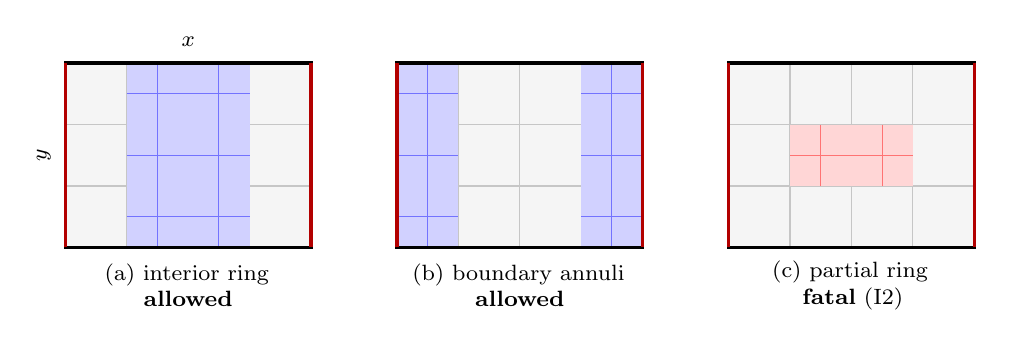
\begin{tikzpicture}[scale=0.78, every node/.style={font=\footnotesize}]
  % ---- allowed: interior ring
  \begin{scope}
    \draw[fill=gray!8] (0,0) rectangle (4,3);
    \foreach \x in {1,2,3} \draw[gray!45] (\x,0) -- (\x,3);
    \foreach \y in {1,2} \draw[gray!45] (0,\y) -- (4,\y);
    % refined ring: column 1..2, full y
    \fill[blue!18] (1,0) rectangle (3,3);
    \foreach \x in {1.5,2.5} \draw[blue!55] (\x,0) -- (\x,3);
    \foreach \y in {0.5,1.5,2.5} \draw[blue!55] (1,\y) -- (3,\y);
    \draw[very thick] (0,0) rectangle (4,3);
    \draw[very thick,red!70!black] (0,0) -- (0,3);
    \draw[very thick,red!70!black] (4,0) -- (4,3);
    \node[text width=3.4cm, align=center] at (2,-0.62) {(a) interior ring\\ \textbf{allowed}};
    \node[rotate=90] at (-0.35,1.5) {$y$};
    \node at (2,3.35) {$x$};
  \end{scope}
  % ---- allowed: boundary annuli
  \begin{scope}[xshift=5.4cm]
    \draw[fill=gray!8] (0,0) rectangle (4,3);
    \foreach \x in {1,2,3} \draw[gray!45] (\x,0) -- (\x,3);
    \foreach \y in {1,2} \draw[gray!45] (0,\y) -- (4,\y);
    \fill[blue!18] (0,0) rectangle (1,3);
    \fill[blue!18] (3,0) rectangle (4,3);
    \foreach \x in {0.5,3.5} \draw[blue!55] (\x,0) -- (\x,3);
    \foreach \y in {0.5,1.5,2.5} {\draw[blue!55] (0,\y) -- (1,\y);
                                  \draw[blue!55] (3,\y) -- (4,\y);}
    \draw[very thick] (0,0) rectangle (4,3);
    \draw[very thick,red!70!black] (0,0) -- (0,3);
    \draw[very thick,red!70!black] (4,0) -- (4,3);
    \node[text width=3.4cm, align=center] at (2,-0.62) {(b) boundary annuli\\ \textbf{allowed}};
  \end{scope}
  % ---- forbidden: partial ring
  \begin{scope}[xshift=10.8cm]
    \draw[fill=gray!8] (0,0) rectangle (4,3);
    \foreach \x in {1,2,3} \draw[gray!45] (\x,0) -- (\x,3);
    \foreach \y in {1,2} \draw[gray!45] (0,\y) -- (4,\y);
    \fill[red!16] (1,1) rectangle (3,2);
    \foreach \x in {1.5,2.5} \draw[red!55] (\x,1) -- (\x,2);
    \draw[red!55] (1,1.5) -- (3,1.5);
    \draw[very thick] (0,0) rectangle (4,3);
    \draw[very thick,red!70!black] (0,0) -- (0,3);
    \draw[very thick,red!70!black] (4,0) -- (4,3);
    \node[text width=3.4cm, align=center] at (2,-0.62) {(c) partial ring\\ \textbf{fatal} (I2)};
  \end{scope}
\end{tikzpicture}
\caption{Refinement policy in the $x$--$y$ plane. Red edges are the shear-periodic
$x_1$ faces. (a) Interior ring: boundary at root level, refinement spans the full
azimuth. (b) Both faces uniformly refined --- allowed by I1 from Phase 0b onward,
and the configuration that creates boundary octets in Phase 2b. (c) A patch that does
not close in $y$ violates I2 whenever orbital advection is on.}
\label{fig:policy}
\end{figure}

\subsection{Where the policy is enforced}
\label{sec:enforce}

Enforcement is deliberately layered: a \emph{veto} that prevents most violations from
being requested, and a \emph{fatal check} that catches anything that slips through.

\begin{center}
\small
\begin{tabular}{@{}llp{6.5cm}@{}}
\toprule
Site & Kind & Effect \\
\midrule
\fn{Mesh::BuildTreeFromScratch} & fatal & I1, I2 checked on the freshly built tree \\
\fn{Mesh::BuildTreeFromRestart} & fatal & Same, on restart \\
\fn{MeshRefinement::CheckForRefinement} & veto & Clears refine flags that would
violate I1 (boundary blocks; graded cap) \\
\fn{MeshRefinement::CheckForRefinement} & sync & Ring-wise OR/AND of flags to enforce
I2 by construction \\
\fn{MeshRefinement::AdaptiveMeshRefinement} & fatal & I1, I2 re-checked after
\fn{RedistAndRefineMeshBlocks} \\
\bottomrule
\end{tabular}
\end{center}

\fn{Mesh::CheckShearingBoxRefinement(ParameterInput*)} (\file{build\_tree.cpp}) is the
single implementation of both invariants. It returns immediately unless the mesh is
multilevel and a \code{<shearing\_box>} block exists. For I1 it scans
\code{lloc\_eachmb} for blocks with $l_{x1} = 0$ or
$l_{x1} = N_{{\rm mb},x1}(\ell) - 1$ and requires
$\ell_{\min} = \ell_{\max}$ over that set. For I2 it accumulates a
\code{std::map} keyed on $(\ell, l_{x1}, l_{x3})$ counting leaf blocks per ring and
requires each count to equal the full azimuthal block count at that level. On a
violation it prints the offending ring and dumps every refined block's logical
location, which is what makes a failed AMR configuration diagnosable at all.

\subsection{The graded refinement cap}
\label{sec:gradedcap}

Vetoing refinement of blocks that \emph{sit} on the boundary is not enough: $2{:}1$
balancing in \fn{UpdateMeshBlockTree} propagates refinement outward from a newly
refined block, and can reach the boundary columns from a few blocks away. Before
commit \code{b5388c02} this turned an over-eager AMR criterion into a fatal abort
mid-run.

The cap is a geometric room requirement. Let $\ell_b$ be the (uniform, by I1) boundary
level and consider a block at level $\ell$ with $s = \ell - \ell_b \ge 1$ requesting
refinement to $\ell+1$. Balancing then requires a buffer column of every intermediate
level between it and the boundary, of total width
$\left(1 - 2^{-s}\right)$ boundary-level columns on each side --- and, expressed in
integer logical coordinates \emph{at the block's own level},
\begin{equation}
  2^{\,s+1} - 1 \;\le\; l_{x1} \;\le\; N_{{\rm mb},x1}(\ell) - 2^{\,s+1}.
  \label{eq:cap}
\end{equation}
The implementation reads exactly that:

\begin{lstlisting}
if (lx1 == 0 || lx1 == (nmbx1-1)) {          // MB on boundary: never refine
  refine_flag.h_view(m+mbs) = 0;
} else if (lev >= (blev+1)) {                // graded cap on interior MBs
  std::int32_t gap = (1 << ((lev-blev)+1));
  if ((lx1 < (gap-1)) || (lx1 > (nmbx1-gap))) { refine_flag.h_view(m+mbs) = 0; }
}
\end{lstlisting}

With the cap in place, any I1 violation surviving to the post-update check is a
genuine bug rather than a criterion asking for too much --- which is what makes it
reasonable to keep that check fatal.

\subsection{Ring-wise flag synchronization}
\label{sec:ringsync}

I2 is enforced \emph{constructively} rather than by veto, immediately after the global
flag \code{Allgatherv} in \fn{CheckForRefinement}. Flags are collapsed into a map keyed
on $(\ell, l_{x1}, l_{x3})$ with the rule
\begin{equation}
  \text{refine if \emph{any} member is flagged;\quad derefine only if \emph{every}
  member is flagged,}
\end{equation}
and then written back to all members of the ring. The "any refine wins" direction
guarantees that a criterion that fires anywhere in a ring produces a complete ring; the
unanimity requirement for derefinement prevents a ring from being partially destroyed.

The ordering matters: this runs \emph{after} the \code{Allgatherv}, on the globally
consistent flag array, so every rank computes the identical map and the result is
deterministic without any additional communication.

\subsection{The derefinement-ordering fix}
\label{sec:sortfix}

Ring-complete derefinement exposed a latent upstream bug. \fn{UpdateMeshBlockTree}
sorts the derefinement-candidate list finest-first so that
\fn{MeshBlockTree::Derefine}'s finer-neighbor veto operates on an already-updated tree,
but used \code{\&cllderef[ctnd-1]} as the end iterator --- excluding the last element:

\begin{lstlisting}
- std::sort(cllderef, &(cllderef[ctnd-1]), Mesh::GreaterLevel);
+ std::sort(cllderef, &(cllderef[ctnd]),   Mesh::GreaterLevel);
\end{lstlisting}

When a mixed-level derefinement left a fine-level parent in the unsorted last slot,
coarser parents merging before it were vetoed \emph{in an order-dependent way}: some
parents of an annulus merged and some did not, splitting what should have been a
ring-complete derefinement and tripping the I2 fatal. Outside the shearing box the
bug only delayed some derefinements by one AMR interval, which is why it had gone
unnoticed.

\subsection{Non-FARGO (full-velocity) mode}
\label{sec:nofargo}

\code{<shearing\_box> orbital\_advection} (default \code{true}) selects the frame.
With \code{false}, \code{OrbitalAdvectionCC}/\code{FC} are simply not constructed
(\code{porb\_u = porb\_b = nullptr}) while the shear-periodic BCs and the Coriolis/tidal
source terms stay active, and the solver integrates the full shear flow directly. This
mode exists for two reasons: it removes constraint I2 entirely (useful for arbitrary
refinement patterns), and it provides an independent frame against which the FARGO
path can be checked.

Consistency requires three coordinated changes.

\paragraph{(i) Source terms (\file{shearing\_box\_srcterms.cpp}).} The shear-subtracted
frame uses the reduced Coriolis coefficient $(2-q)\Om$ on $\dot{m}_2$ because the
background shear's contribution is carried analytically by orbital advection. In the
full-velocity frame the velocities \emph{include} the background, so the code applies
the full Coriolis force plus the radial tidal force:
\begin{equation}
  \dot{m}_1 \mathrel{+}= 2\Om m_2, \qquad
  \dot{m}_2 \mathrel{-}= 2\Om m_1, \qquad
  \dot{m}_1 \mathrel{+}= 2q\Om^2 \rho\, x ,
\end{equation}
with the corresponding tidal work added to the total energy for an ideal EOS.

\paragraph{(ii) Boundary momentum/energy offsets (\file{shearing\_box\_cc.cpp}).} The
background azimuthal velocity jumps by $\qom L_x$ across the box, so data wrapped
through the shear-periodic boundaries must be offset to represent the \emph{local}
frame. After the unpack, for each ghost cell:
\begin{equation}
  E \mathrel{+}= \delta v_y\, m_2 + \tfrac{1}{2}\rho\, \delta v_y^2, \qquad
  m_2 \mathrel{+}= \rho\, \delta v_y, \qquad
  \delta v_y = \begin{cases} +\qom L_x & \text{at } ix_1 \\
                             -\qom L_x & \text{at } ox_1 \end{cases}
\end{equation}
Note the order: energy uses the pre-update $m_2$, so the momentum update must come
second.

\paragraph{(iii) Initial conditions (\file{shwave.cpp}, \file{swing.cpp}).} Every
problem generator branch adds $v_y^{(0)} = -\qom x$ to the initial azimuthal velocity
when \code{orbital\_advection = false}, with the matching kinetic-energy contribution.

\paragraph{MHD restriction.} MHD orbital advection remaps face-centered $B$ through
EMFs; the correctness of that remap at fine/coarse interfaces (specifically,
$\nabla\!\cdot\!B$ preservation) has not been analyzed, so MHD $+$ FARGO $+$
refinement remains fatal in \fn{MHD::MHD}. Hydro is supported, and MHD without
orbital advection is supported.

\subsection{The shift-depth estimate and its runtime guard}
\label{sec:maxjshift}

Orbital advection communicates a buffer of depth $\code{ng} + \code{maxjshift}$, where
\code{maxjshift} is estimated once at construction. The original estimate,
$\lceil \mathrm{CFL} \cdot \max|x_1| \rceil$, omitted the $\qom$ factor. It was
corrected to
\begin{equation}
  \code{maxjshift} = \left\lfloor \mathrm{CFL}\,(\qom)\max|x_1| \right\rfloor + 1,
  \qquad \text{doubled on multilevel meshes,}
\end{equation}
the doubling being headroom for fine blocks at large $|x_1|$, whose shift in their own
(smaller) cell units is larger whenever $\Delta t$ is not set by that same region.

Because that is still a heuristic, \fn{OrbitalAdvectionCC::RecvAndUnpackCC} now
\emph{verifies} it every step against this step's $\Delta t$ and each block's own
geometry, before unpacking:
\begin{equation}
  \max_m \left\lfloor \frac{\qom \Delta t\, \max|x_1|_m}{\Delta x_{2,m}} \right\rfloor
  \;\le\; \code{maxjshift},
\end{equation}
aborting with a message that names the observed shift and the buffer depth. This
converts a silent out-of-bounds read into a diagnosable failure.

\subsection{Phase 0c: making the boundary state rebuildable under AMR}
\label{sec:amrreinit}

AMR renumbers MeshBlock GIDs and reassigns blocks to ranks on every update, but
\code{x1bndry\_mbgid}, the MPI request arrays, and the send/recv buffers were all built
once in the \code{ShearingBox} constructor. Running AMR would have silently corrupted
the shear exchange. The restructuring:

\begin{center}
\small
\begin{tabular}{@{}lp{9.3cm}@{}}
\toprule
\fn{ShearingBox::SetX1BndryMBs()} & List and request-array construction, extracted
from the constructor and re-expressed against \code{pmy\_pack} so it can run on the
current pack. Grow-only \code{realloc} of \code{x1bndry\_mbgid}; all requests reset to
\code{MPI\_REQUEST\_NULL}. \\
\fn{ShearingBox::AllocateBuffers()} & New pure virtual; \code{ShearingBoxCC} and
\code{ShearingBoxFC} override it with the grow-only buffer reallocation extracted from
their constructors. \code{ShearingBoxCC} now stores \code{nvar} because it needs it to
size buffers outside the constructor. \\
\fn{ShearingBox::ReinitAfterMeshUpdate()} & \fn{SetX1BndryMBs()} followed by the
virtual \fn{AllocateBuffers()}. \\
\bottomrule
\end{tabular}
\end{center}

\noindent
The call site is \fn{MeshRefinement::AdaptiveMeshRefinement}, placed after
\fn{RedistAndRefineMeshBlocks} and the post-update policy check, and \emph{before}
\fn{InitBoundaryValuesAndPrimitives} --- i.e.\ after the block metadata is rebuilt and
before any boundary exchange touches the new mesh. It fires for
\code{phydro->psbox\_u}, \code{pmhd->psbox\_u}, and \code{pmhd->psbox\_b} when present.

The communicator is created once (\code{MPI\_Comm\_dup} in the constructor) and not
re-duplicated; only the request arrays and buffers are rebuilt. Buffers grow but never
shrink, which avoids reallocation churn when the block count oscillates; the extra
slots are simply unused.

\subsection{A user AMR criterion for testing: the moving ring}
\label{sec:movingring}

Exercising ring creation and destruction requires a criterion whose behavior is known
in advance. \fn{MovingRingRefine} (in \file{shwave.cpp}; an identical
\fn{SwingMovingRingRefine} in \file{swing.cpp}) refines every block whose $x_1$ extent
overlaps
\begin{equation}
  \left[x_c(t) - w,\; x_c(t) + w\right], \qquad
  x_c(t) = x_{c0} + x_{\rm amp}\sin(\omega_r t),
\end{equation}
and flags all others for derefinement. Because the criterion depends only on $x_1$ it
naturally flags complete rings; the ring sync and boundary vetoes of
\S\ref{sec:enforce} supply the rest of the policy. It runs on host data (block bounds
only, no kernel) and is enrolled from the problem generator on both fresh starts and
restarts, controlled by \code{<problem> amr\_moving\_ring} and the parameters
\code{ring\_xc0}, \code{ring\_xamp}, \code{ring\_freq}, \code{ring\_hwidth}.

Two practical consequences of user-criterion AMR are worth recording, because they
constrain what tests can prove: a run starts on the \emph{unrefined} root mesh and
refines within the first \code{refinement\_interval} cycles, so bit-identity with an
equivalent SMR run is structurally impossible; and \code{max\_nmb\_per\_rank} must
carry transient headroom for the moment when the old ring has not yet been destroyed
and the new one already exists.

%=========================================================================================
\section{Phase 1: shear-periodic boundaries for the multigrid solver}
\label{sec:phase1}

\subsection{The design decision}

Equation~\eqref{eq:shearid} is an identification of the domain with its azimuthally
displaced image. It changes \emph{which cells are neighbors}, not \emph{what the
operator is}. So:

\invariant{Design rule.}{The 7-point Laplacian, the smoother, the restriction and
prolongation operators, and the coarse-grid solve are untouched. Shear-periodicity
enters exclusively as a modified $x_1$ ghost fill --- one that shifts the incoming
plane by $\pm\, q\Om t_s L_x$ in $y$ --- applied identically at every level of the
multigrid hierarchy.}

\noindent
Two properties of multigrid make the "identically at every level" clause cheap.
First, the FAS V-cycle's fixed point satisfies the \emph{finest}-level system; the
coarse levels only accelerate convergence. Coarse-level remap quality therefore
affects the convergence \emph{rate}, not the answer. Second, because the shift is
generally a non-integer number of cells at \emph{every} level anyway, no level is a
special case: one code path serves all of them.

\subsection{The shear phase \texorpdfstring{$q\Om t_s$}{qOmt}}

The box is strictly shear-periodic at times $t_n = n L_y / (\qom L_x)$; measuring the
offset from the most recent such instant keeps the shift --- and hence the remap
error --- minimal:

\begin{lstlisting}
Real MultigridDriver::ComputeShearQomt(Real time) const {
  Real tshear = ly/(mg_qshear_*mg_omega0_*lx);
  Real dts = time - std::floor(time/tshear)*tshear;
  return mg_qshear_*mg_omega0_*dts;
}
\end{lstlisting}

\fn{MGGravityDriver::Solve} freezes \code{mg\_qomt\_} once per solve, from
\code{pmesh->time}. This is deliberately the \emph{same convention as the FFT solver},
so both solvers see identical boundary identifications at any instant and can be
compared bit-for-bit. Note that hydro's own shear-periodic BC uses \code{time+dt} on
the final RK stage; the resulting $O(\Delta t)$ offset between gravity and hydro is a
pre-existing, FFT-validated convention and is intentionally \emph{not} "fixed" in the
multigrid path, since doing so would break the solver-to-solver comparison that
validates it.

\subsection{Data structures}

Two members are added to \code{Multigrid} (\file{multigrid.hpp}):

\begin{center}
\small
\begin{tabular}{@{}lp{9.4cm}@{}}
\toprule
\code{DvceArray4D<Real> *shear\_plane\_} & One global boundary plane per multigrid
level, dimensioned \code{(2, nvar*ngh, gnz, gny)}. Index 0 selects the face: plane
0 is the \emph{source for the inner ghosts} (gathered at the outer boundary), plane 1
the source for the outer ghosts. \\
\code{DvceArray2D<int> shear\_goffs\_} & Per-block global $(y,z)$ cell offsets at the
finest level, $(l_{x2}n_{x2},\, l_{x3}n_{x3})$, shifted right by the level index at
use. \\
\code{int shear\_reflev\_} & Refinement offset of the $x_1$-boundary blocks above root
(Phase 2b; zero on uniform grids and interior-only refinement). \\
\bottomrule
\end{tabular}
\end{center}

\noindent
and four on \code{MultigridDriver}: \code{mg\_shear\_enabled\_},
\code{mg\_qshear\_}/\code{mg\_omega0\_}, \code{mg\_qomt\_} (frozen per solve), and
\code{mg\_remap\_order\_}.

Plane extents at level $l$ (with $\code{ll} = \code{nlevel\_}-1-l$) are
\begin{equation}
  \code{gny} = \left(N_{{\rm mb},x2} \ll \code{shear\_reflev\_}\right)
               \left(n_{x2} \gg \code{ll}\right), \qquad
  \code{gnz} = \left(N_{{\rm mb},x3} \ll \code{shear\_reflev\_}\right)
               \left(n_{x3} \gg \code{ll}\right),
\end{equation}
i.e.\ the full $y$--$z$ extent of the mesh at the boundary blocks' level, coarsened to
this multigrid level.

\subsection{The block-level fill: gather, remap, scatter}
\label{sec:fillpack}

\fn{Multigrid::FillShearGhostPack(qomt, order)} is three kernels submitted on one
execution-space instance --- stream-ordered, so no explicit fences are required
between them.

\begin{figure}[htb]
\centering
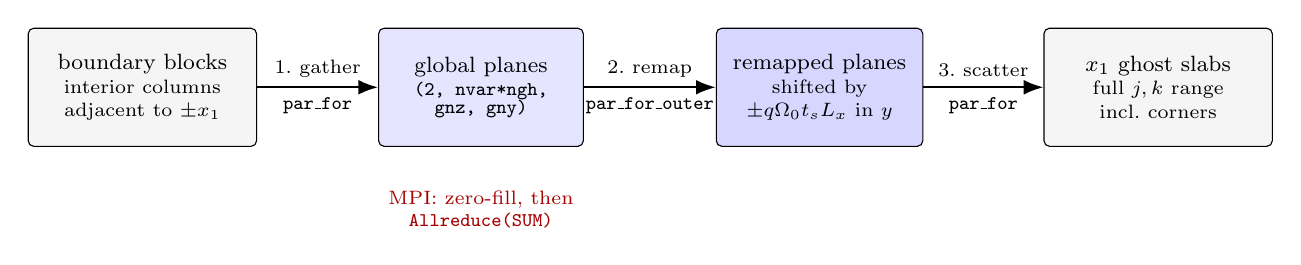
\begin{tikzpicture}[
  every node/.style={font=\footnotesize},
  box/.style={draw, rounded corners=2pt, minimum height=1.5cm, align=center,
              inner sep=6pt},
  ar/.style={-{Latex[length=2.5mm]}, thick}]
  \node[box, fill=gray!8, minimum width=2.9cm] (blk) at (0,0)
    {boundary blocks\\[-1pt]\scriptsize interior columns\\[-1pt]
     \scriptsize adjacent to $\pm x_1$};
  \node[box, fill=blue!10, minimum width=2.6cm] (pl) at (4.3,0)
    {global planes\\[-1pt]\scriptsize \code{(2, nvar*ngh,}\\[-3pt]
     \scriptsize \code{gnz, gny)}};
  \node[box, fill=blue!16, minimum width=2.6cm] (pl2) at (8.6,0)
    {remapped planes\\[-1pt]\scriptsize shifted by\\[-1pt]
     \scriptsize $\pm q\Om t_s L_x$ in $y$};
  \node[box, fill=gray!8, minimum width=2.9cm] (gh) at (12.9,0)
    {$x_1$ ghost slabs\\[-1pt]\scriptsize full $j,k$ range\\[-1pt]
     \scriptsize incl.\ corners};
  \draw[ar] (blk) -- node[above]{\scriptsize 1.\ gather}
                    node[below]{\scriptsize \code{par\_for}} (pl);
  \draw[ar] (pl) -- node[above]{\scriptsize 2.\ remap}
                   node[below]{\scriptsize \code{par\_for\_outer}} (pl2);
  \draw[ar] (pl2) -- node[above]{\scriptsize 3.\ scatter}
                    node[below]{\scriptsize \code{par\_for}} (gh);
  \node[align=center, font=\scriptsize] at (4.3,-1.55)
    {\textcolor{red!65!black}{MPI: zero-fill, then}\\
     \textcolor{red!65!black}{\code{Allreduce(SUM)}}};
\end{tikzpicture}
\caption{The block-level shear ghost fill. The only MPI seam is a single
\code{Allreduce} between gather and remap.}
\label{fig:fill}
\end{figure}

\paragraph{1. Gather.} Over all blocks and all interior $(k,j)$, blocks whose
\code{mb\_bcs} carries \code{shear\_periodic} on an $x_1$ face write their \code{ngh}
interior columns adjacent to that face into the plane at global index
$(\code{gk},\code{gj})$ derived from \code{shear\_goffs\_}. Note the crossing: an
\emph{outer}-boundary block feeds plane 0, which will fill \emph{inner} ghosts.
Non-boundary blocks --- including all interior fine blocks under Phase 2a --- are
skipped by the \code{mb\_bcs} test, with no extra logic.

\paragraph{2. Remap.} A team kernel over $(\text{face}\times\text{var}\times\text{depth},\;
\code{gk})$. For each row, the shift $y_{\rm sh} = \pm\, q\Om t_s L_x$ is split:
\begin{equation}
  \code{joffset} = \left\lfloor y_{\rm sh}/\Delta y_l \right\rfloor, \qquad
  \epsilon = \operatorname{fmod}(y_{\rm sh}, \Delta y_l)/\Delta y_l .
\end{equation}
The integer part is folded into a \emph{periodic-wrapped scratch load}
$q_{jf} = \text{plane}[(jf - \code{PAD} - \code{joffset}) \bmod \code{gny}]$, and the
fractional part is applied by the shared conservative kernels via
Eq.~\eqref{eq:remap}. Because a full period is loaded before any write-back, the
remap is safely in-place.

The scratch padding is \code{PAD = 3}: PPMX reads $j-2 \dots j+2$ plus the face at
$ju+1$, so three is exactly sufficient --- and, crucially, independent of the shift
size, because the integer part never enters the stencil. This is why $\code{ngh} = 1$
imposes no stencil limitation on the multigrid solver even though the shift can be
many cells.

\paragraph{3. Scatter.} Over the \emph{full} slab $k,j \in [0,\, \code{ncells}+2\code{ngh})$
--- not just interior cells --- with periodic wrap in $y$ and $z$. Writing the slab's
edge and corner ghosts matters: trilinear prolongation reads them. The read set
(interior columns) and write set (ghost columns) are disjoint, so gather and scatter
cannot race.

\subsection{The root-grid fill}

The root grid is a single replicated global array, so it needs no planes and is
remapped in place by \fn{MultigridDriver::RootShearBoundaryX1}, a single team kernel
that loads the source column with the wrapped offset, applies the same remap fluxes,
and writes the destination ghost column. It fills the interior-row ghosts only; the
$x_2$/$x_3$ passes of \fn{MGRootBoundary} that follow supply the ghost-corner rows by
periodic wrap of these already-remapped rows. At $q\Om t_s = 0$ it reduces exactly to
the plain periodic copy, because the remap fluxes vanish identically at $\epsilon = 0$
--- which is what makes the "shear-periodic instant equals periodic, bitwise" test
meaningful.

\subsection{Hooks into the existing solver}
\label{sec:hooks}

\begin{center}
\small
\begin{tabular}{@{}>{\raggedright\arraybackslash}p{7.1cm}p{7.4cm}@{}}
\toprule
Call site (file) & What it does \\
\midrule
\fn{MultigridDriver::MultigridDriver}\newline
\hspace*{1em}\file{multigrid\_driver.cpp} &
\code{shear\_periodic} is kept as its own \code{mg\_mesh\_bcs\_} value instead of
collapsing to \code{mg\_zerofixed} \\[2pt]
\fn{MGGravityDriver::MGGravityDriver}\newline
\hspace*{1em}\file{mg\_gravity.cpp} &
Enables shear, reads parameters, applies guards, calls \fn{AllocateShearPlanes} \\[2pt]
\fn{MGGravityDriver::Solve}\newline
\hspace*{1em}\file{mg\_gravity.cpp} & Freezes \code{mg\_qomt\_} once per solve \\[2pt]
\fn{MultigridDriver::PhysicalBoundary}\newline
\hspace*{1em}\file{multigrid\_tasks.cpp} &
Calls \fn{FillShearGhostPack} after every boundary exchange \\[2pt]
\fn{MultigridDriver::MGRootBoundary}\newline
\hspace*{1em}\file{multigrid\_driver.cpp} &
Calls \fn{RootShearBoundaryX1} before the $x_1/x_2/x_3$ passes \\[2pt]
\fn{MultigridDriver::InitializeOctets}\newline
\hspace*{1em}\file{multigrid\_driver.cpp} &
\code{shear\_periodic} wraps like periodic in the neighbor search \\[2pt]
\fn{ApplyPhysicalBoundariesOctet}\newline
\hspace*{1em}\file{multigrid\_driver.cpp} &
\code{shear\_periodic} is a wrap, not a wall: no reflection applied \\
\bottomrule
\end{tabular}
\end{center}

\noindent
The ordering rule at every one of these sites is the same: \emph{the shear fill runs
after the ordinary (unsheared) exchange and overwrites its result}. The exchange
performs the plain periodic copy through the neighbor tables; the shear fill replaces
that copy with the $y$-remapped image over the whole slab. This is why the fill is
placed at the top of \fn{PhysicalBoundary}, which is the point every boundary
exchange funnels through --- including the final finest-level exchange that feeds
\code{SelfGravity}'s $\phi$ ghosts.

\subsection{Two corrections uncovered by the plumbing}

\paragraph{The \code{mg\_zerofixed} fall-through.} Before this work,
\code{shear\_periodic} was not a recognized multigrid BC and fell through to
\code{mg\_zerofixed}. The consequence was severe and silent: the communication's
(correct, unsheared) periodic copy was overwritten with a $\Phi = 0$ Dirichlet wall,
and mean-source subtraction was disabled because the domain no longer looked fully
periodic. Shearing-box multigrid gravity ran silently wrong. Recognizing
\code{shear\_periodic} throughout \code{mg\_mesh\_bcs\_} fixes both.

\paragraph{Mean-source subtraction.} A fully periodic Poisson problem is solvable only
if the source has zero mean. \code{shear\_periodic} is a periodic identification, not
a physical boundary, so it must count toward "fully wrapped":

\begin{lstlisting}
bool wrap_all = true;
for (int f = 0; f < 6; ++f) {
  BoundaryFlag mbc = pmy_mesh_->mesh_bcs[f];
  wrap_all = wrap_all && (mbc == BoundaryFlag::periodic ||
                          mbc == BoundaryFlag::shear_periodic);
}
if (!wrap_all) { fsubtract_average_ = false; }
\end{lstlisting}

\subsection{Driver-independent task-list execution}

Multigrid task lists were run through \fn{Driver::ExecuteTaskList}, which
dereferences the \code{Driver*}. Problem generators are constructed \emph{before} the
\code{Driver} exists, so a static Poisson solve from a pgen
(\code{pgrav->Solve(nullptr, 1)}) crashed with \code{solver = multigrid}.
\fn{MultigridDriver::ExecuteMGTaskList} replicates the runner but tolerates
\code{pdriver == nullptr}, which is safe because every multigrid task ignores its
\code{Driver*} argument. Together with a null guard in the non-convergence branch of
\fn{SolveIterative}, this makes static solves through the full multigrid path a
supported configuration --- the mechanism behind the static Poisson tests.

\subsection{The MPI seam}
\label{sec:mpiseam}

Multi-rank support required exactly one collective, at one place
(Fig.~\ref{fig:fill}). Each rank gathers only its own boundary blocks' columns into a
zero-filled plane; one \code{MPI\_Allreduce(MPI\_IN\_PLACE, ..., MPI\_SUM)} then
reconstructs the global plane on every rank; remap and scatter proceed rank-locally
(redundantly, but the planes are small).

Two properties make this exact rather than merely adequate. First, every plane cell
has \emph{exactly one} writer --- boundary blocks tile the level's $y$--$z$ extent ---
so the summed contributions are one value plus zeros, and the result is independent of
reduction order: the multi-rank solve is bit-identical to the serial one. Second, all
ranks reach the collective in lockstep, because every early-return at the call site
(\code{shear\_plane\_ == nullptr}, \code{ncells < 1}, \code{mg\_qomt\_ == 0}) is a
level-global condition, not a rank-local one. The \code{Kokkos::fence()} before the
call is required because the gather kernel is asynchronous.

The root grid needs no communication (it is replicated), and the octet fill of Phase 2b
needs none either (octets are replicated). The seam is compiled out entirely in serial
builds.

The same commit made the \file{fft\_poisson} pgen's diagnostics MPI-aware: the density
mean and all residual/error norms were rank-local reductions written under the FFT
solver's single-rank assumption, which corrupted the printed RHS mean and scaled the
$L_2$ norms by $1/\sqrt{N_{\rm ranks}}$ under MPI.

\subsection{Phase-1 guards and parameters}

\begin{center}
\small
\begin{tabular}{@{}lp{8.3cm}@{}}
\toprule
Condition & Reason \\
\midrule
$x_2$ or $x_3$ not periodic & The shear identification assumes a periodic azimuth and
vertical; the plane wrap would be wrong \\
\code{<gravity> mg\_bc} set & An explicit MG boundary override cannot be combined with
the shear identification \\
\code{root\_on\_host = true} & The root shear fill is a device kernel \\
\code{mg\_nghost > 1} & Untested; also the octet fill of Phase 2b assumes
$\code{ngh}=1$ (octet interiors are 2 cells) \\
\code{mg\_remap} unrecognized & Must be \code{dc}, \code{plm} (default), or \code{ppmx} \\
\bottomrule
\end{tabular}
\end{center}

%=========================================================================================
\section{Phase 2: multigrid gravity on refined shearing-box meshes}
\label{sec:phase2}

Phase 2 is decomposed into three steps chosen so that each one isolates a single new
mechanism, and each can be validated against the previous step as a regression.

\begin{center}
\small
\begin{tabular}{@{}lll@{}}
\toprule
Step & Mesh configuration & New mechanism \\
\midrule
2a & Interior rings; boundary at root level & none (guard relaxation) \\
2b & Boundary annuli; both faces refined uniformly & sheared \emph{octet} ghosts \\
2c & Adaptive refinement & rebuild-on-remesh \\
\bottomrule
\end{tabular}
\end{center}

\subsection{Phase 2a: interior rings}
\label{sec:phase2a}

Phase 2a required \emph{no changes to the fill at all}, and understanding why is the
point of the step.

The shear fill iterates over blocks and gates on \code{mb\_bcs}. Interior fine blocks
do not carry \code{shear\_periodic} on any $x_1$ face, so the gather and scatter skip
them automatically. Every \emph{participating} block is at the root level, so the
plane geometry --- sized in root-block units at construction --- remains correct. The
refined interior is handled entirely by the pre-existing octet machinery, which is
level-agnostic and does not touch the shear faces.

What changed was the guard. The Phase-1 blanket \code{multilevel} fatal became a
scan requiring every block on an $x_1$ face to be at the root level, with AMR still
fatal (deferred to 2c) and refined boundary faces still fatal (deferred to 2b).

\subsection{Phase 2b: sheared octet ghosts}
\label{sec:phase2b}

Boundary annuli --- both $x_1$ faces uniformly refined over their full $x_2$/$x_3$
extent, allowed by I1 since Phase 0b --- put multigrid \emph{octets} on the
shear-periodic faces. Those octets exchange $x_1$ ghosts through the octet neighbor
table, which wraps periodically (\fn{InitializeOctets}, patched in Phase 1) but
\emph{unsheared}. They need the same treatment as the blocks.

\paragraph{Why this is a separate implementation.} The octet regime differs from the
block regime in every respect that matters to the fill: octet buffers live in
\emph{host} memory, are \emph{replicated on every rank}, and have a fixed $2^3$
interior. So \fn{FillShearOctetGhosts} is the Phase-1 algorithm --- gather, remap,
scatter, same sign convention --- re-expressed as serial host code over a
\code{std::vector} plane, with no MPI seam at all.

\paragraph{The scalar remap twins.} The conservative remap kernels are Kokkos
\emph{team} kernels and cannot be called from serial host code. Rather than
duplicate the reconstruction logic, \file{remap\_fluxes.hpp} gains scalar per-face
twins --- \fn{DC\_RemapFlxFace}, \fn{PLM\_RemapFlxFace}, \fn{PPMX\_RemapFlxFace} ---
each returning the remap flux at one face of a padded row, with the same convention as
the team versions (faces $jf \in [\code{PAD},\, \code{PAD}+\code{gny}]$). The
upwind cell is $c = jf-1$ for $\epsilon > 0$ and $c = jf$ for $\epsilon < 0$, matching
which face the team kernels write. The device path is untouched, which is what
preserves the Phase-1 and Phase-2a results bit-for-bit.

The header carries an explicit maintenance rule: \emph{the math must stay in lockstep
with the team versions; any change to one is a change to both}.

\paragraph{Gating.} \code{oct\_shear\_face\_} is a per-octet-level flag set in
\fn{InitializeOctets}: level $l$ is flagged when its octets reach \emph{both}
$l_{x1} = 0$ and $l_{x1} = (\code{nrbx1\_} \ll l) - 1$. Under I1 either both faces are
tiled at a level or neither is, so a single boolean per level is sufficient.

\paragraph{Hook points.} Every consumer of octet ghosts funnels through two
chokepoints, and the fill is placed at both, after the per-octet exchange:
\begin{itemize}\itemsep2pt
\item \fn{SetBoundariesOctets(fprolong, folddata)} --- per level, during the cycle:
      \code{FillShearOctetGhosts(lev, folddata)};
\item \fn{SetOctetBoundariesBeforeTransfer(folddata)} --- all levels, before the
      root transfer, since these ghosts feed \fn{SetFromRootGrid} for the boundary
      blocks' coarsest levels.
\end{itemize}
The \code{folddata} argument propagates to the fill: when set, \code{Uold} is
gathered, remapped, and scattered alongside \code{U} in the same pass (the plane
carries a leading \code{nfield} axis of size 1 or 2).

\paragraph{Plane sizing at the boundary level.} With boundary annuli the participating
blocks sit at a uniform level \emph{above} root, so the block planes must span the
$y$--$z$ extent at \emph{that} level. \fn{AllocateShearPlanes} determines it by
scanning for the first block on an $x_1$ face --- under I1, any face block gives the
answer --- and stores $\code{shear\_reflev\_} = \ell - \ell_{\rm root}$, which then
multiplies \code{gny} and \code{gnz}.

\paragraph{Guard relaxation.} The 2a root-level requirement weakens to exactly the
hydro invariant I1: the $x_1$-face blocks must share one uniform level, reported with
the observed level span on violation. Interior rings (boundary at root) and boundary
annuli (boundary above root) both pass through the same check.

\paragraph{A note on coarse-level fidelity.} As in Phase 1, the V-cycle's fixed point
is set by the finest block level, so octet-level ghost quality affects only the
convergence rate. The fill is still done consistently at every octet level, because an
inconsistent coarse-grid correction is what would degrade the sheared contraction
factor away from its periodic value.

\subsection{Phase 2c: adaptive refinement}
\label{sec:phase2c}

AMR invalidates every shear structure that was sized at construction: plane extents
(if the boundary level changes), the per-block offset table (load balancing can
reassign blocks without changing their count), and the octet face flags.

The fix rides machinery that already exists. \fn{MultigridDriver::PrepareForAMR} is
called at the top of every \fn{Solve} and already detects any remesh via an update
counter, rebuilding the multigrid arrays and $\phi$. Two changes complete the picture:

\begin{enumerate}\itemsep3pt
\item \fn{Multigrid::AllocateShearPlanes} is made \emph{idempotent}: the plane array
      is allocated only if null, \code{Kokkos::realloc} resizes each plane if the
      boundary level changed, \code{shear\_reflev\_} is re-derived, and the offset
      table is recomputed from the current logical locations. It is then called from
      the same rebuild branch of \fn{PrepareForAMR}.
\item The octet face flags need no new code: \fn{InitializeOctets} is already part of
      the rebuild and reassigns \code{oct\_shear\_face\_} from the new octet set.
\end{enumerate}

\noindent
The constructor's \code{adaptive} fatal is removed. The invariant it was protecting is
not abandoned but relocated: \fn{Mesh::CheckShearingBoxRefinement} re-enforces I1 and
I2 after \emph{every} AMR update (\S\ref{sec:enforce}), so by the time
\fn{PrepareForAMR} runs, the mesh is known to satisfy the uniform-boundary-level
condition that the plane sizing assumes.

Finally, the swing problem generator gains the moving-ring criterion of
\S\ref{sec:movingring}, so that AMR $+$ shear $+$ multigrid gravity can be exercised
on a problem with a known analytic reference.

\subsection{End-to-end control flow}

\begin{figure}[htb]
\centering
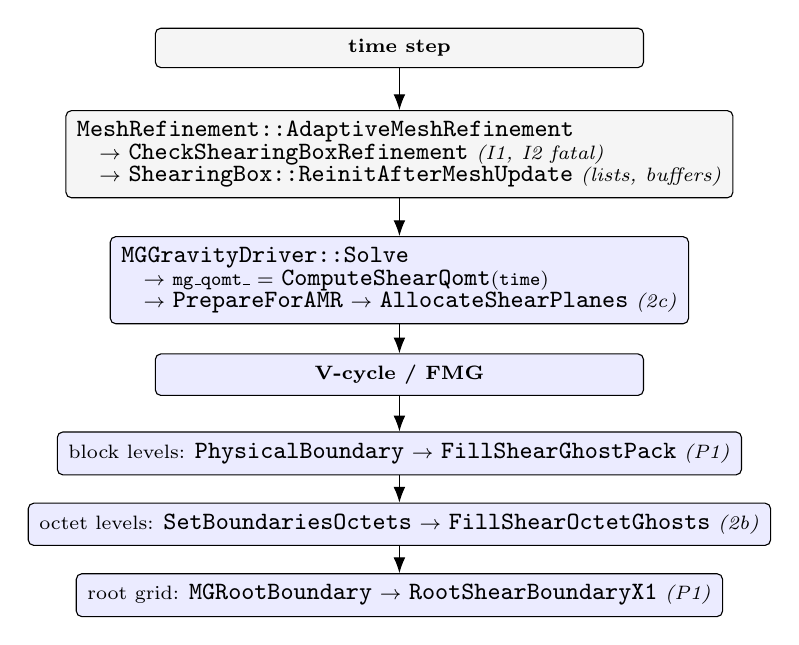
\begin{tikzpicture}[
  every node/.style={font=\scriptsize},
  st/.style={draw, rounded corners=2pt, align=left, inner sep=4pt,
             minimum width=6.2cm},
  hy/.style={st, fill=gray!8},
  mg/.style={st, fill=blue!8},
  ar/.style={-{Latex[length=2mm]}}]
  \node[hy] (a) at (0,0)
    {\textbf{time step}};
  \node[hy] (b) at (0,-1.35)
    {\fn{MeshRefinement::AdaptiveMeshRefinement}\\
     \hspace{1em}$\rightarrow$ \fn{CheckShearingBoxRefinement} \textit{(I1, I2 fatal)}\\
     \hspace{1em}$\rightarrow$ \fn{ShearingBox::ReinitAfterMeshUpdate} \textit{(lists, buffers)}};
  \node[mg] (c) at (0,-2.95)
    {\fn{MGGravityDriver::Solve}\\
     \hspace{1em}$\rightarrow$ \code{mg\_qomt\_} $=$ \fn{ComputeShearQomt}(\code{time})\\
     \hspace{1em}$\rightarrow$ \fn{PrepareForAMR} $\rightarrow$ \fn{AllocateShearPlanes}
     \textit{(2c)}};
  \node[mg] (d) at (0,-4.15)
    {\textbf{V-cycle / FMG}};
  \node[mg] (e) at (0,-5.15)
    {block levels: \fn{PhysicalBoundary}
     $\rightarrow$ \fn{FillShearGhostPack} \textit{(P1)}};
  \node[mg] (f) at (0,-6.05)
    {octet levels: \fn{SetBoundariesOctets}
     $\rightarrow$ \fn{FillShearOctetGhosts} \textit{(2b)}};
  \node[mg] (g) at (0,-6.95)
    {root grid: \fn{MGRootBoundary}
     $\rightarrow$ \fn{RootShearBoundaryX1} \textit{(P1)}};
  \draw[ar] (a) -- (b);  \draw[ar] (b) -- (c);  \draw[ar] (c) -- (d);
  \draw[ar] (d) -- (e);  \draw[ar] (e) -- (f);  \draw[ar] (f) -- (g);
\end{tikzpicture}
\caption{Where each piece runs. Grey: mesh/hydro side (Phase 0). Blue: multigrid
solver (Phases 1--2).}
\label{fig:flow}
\end{figure}

%=========================================================================================
\section{Phase 3: the stratified box --- vertical gravity, slab-open multigrid
boundaries, and cooling}
\label{sec:phase3}

Phases 0--2 built refinement and multigrid self-gravity for the \emph{unstratified}
shearing box: gravity was solved on a fully (shear-)periodic domain, which is why mean
subtraction (the Jeans swindle) was mandatory and why every boundary of the Poisson
problem was an identification rather than a physical edge. Phase 3 adds the third
dimension of the physical problem: vertical stratification. The target application is
the gravito-turbulent disk of Shi \& Chiang (2014, ApJ 789, 34; hereafter SC14) ---
a 3D, stratified, self-gravitating, cooling shearing box --- which requires four new
ingredients: (i) the work term of the vertical tidal force in the energy equation,
(ii) an \emph{open (vacuum) vertical boundary condition} for the multigrid Poisson
solver on a horizontally (shear-)periodic box, (iii) optically thin cooling source
terms, and (iv) a problem generator with SC14's self-gravitating hydrostatic initial
state and diagnostics.

\subsection{Phase 3a: hydro-side stratification terms}
\label{sec:phase3a}

\paragraph{The missing energy work term.} The momentum-side vertical tidal force
$-\rho\Om^2 z\,\hat z$ already existed behind \code{<shearing\_box>
stratified\,=\,true}, but the corresponding work term in the energy equation ---
$-\rho\Om^2 z\,v_z$, cf.\ SC14 eq.~(3) --- was absent in all four source-term
branches (hydro/MHD $\times$ FARGO/non-FARGO). For isothermal runs (the only
stratified configurations exercised upstream) this is invisible; for an ideal-gas
stratified box it is a first-order energy error. All four branches now apply
\begin{equation}
  \Delta E = -\,\Delta t\,\rho\,\Om^2 z\, v_z ,
\end{equation}
consistent with the existing convention of building source terms from primitives.

\paragraph{Cooling.} Two SC14 prescriptions were added to \code{SourceTerms}
(\file{srcterms/srcterms.cpp}), both operating on the internal energy density $U$:
\begin{align}
  \code{beta\_cooling}&: & \dot U &= -\,U\,\Om/\beta ,
    & \beta &= \code{bcool\_beta} \;(=\Om t_{\rm cool}), \\
  \code{thermal\_cooling}&: & \dot U &= -\,U/t_{\rm cool}, &
    t_{\rm cool} &= b\,(\rho/P)^3 \quad (\code{tcool\_b}),
\end{align}
the second being SC14's optically thin constant-opacity law (their eq.~8).
$\Om$ defaults to \code{<shearing\_box>~omega0}. \fn{SourceTerms::NewTimeStep} caps
the step at $\code{cool\_eps}\,t_{\rm cool}$ (default $0.02$, SC14's choice); for
\code{beta\_cooling} the cap is a constant and never binds in practice.

\paragraph{Vertical hydro boundaries: diode, not outflow.} SC14 describe their
vertical boundaries as ``outflow.'' With AthenaK's plain \code{outflow} BC (ghost =
copy of the last active cell) the stratified box is \emph{unstable to an inflow
runaway}: once gravity establishes an inward velocity at the $z$ faces, the copied
ghost state feeds mass at that velocity indefinitely. In the hydrostatic-hold test
below, the halo density grew by two orders of magnitude in $10\,\Om^{-1}$ and the
accreting fountain destroyed the disk. The \code{diode} BC (outflow that zeroes
inbound normal velocity in the ghosts) removes the reservoir; the reference inputs
use it on both $z$ faces.

\subsection{Phase 3b: slab-open vertical boundaries for the multigrid solver}
\label{sec:phase3b}

\paragraph{Problem statement.} The Poisson problem of the stratified box is
(shear-)periodic in $x_1$, periodic in $x_2$, and \emph{open} in $x_3$: the correct
exterior solution is vacuum decay, mode by horizontal mode. The FFT solver already
provides this configuration via the Koyama \& Ostriker (2009) two-solve method
(\code{vert\_bc\,=\,open}), but only on uniform single-rank grids; making the
\emph{multigrid} solver support it is what buys refinement compatibility.

\paragraph{Method: exact Dirichlet face planes from the discrete vacuum Green's
function.} For each horizontal Fourier mode of the rolled (strictly periodic) frame,
with discrete horizontal eigenvalue
\begin{equation}
  \lambda_\perp = \frac{2\cos(k_x'\Delta x_1)-2}{\Delta x_1^2}
                + \frac{2\cos(k_y \Delta x_2)-2}{\Delta x_2^2} \le 0 ,
  \qquad k_x' = k_x + q\Om t_s \tfrac{L_x}{L_y}k_y ,
\end{equation}
the 7-point stencil reduces in $z$ to a three-term recurrence whose decaying solution
is $\mu^{|\Delta n|}$ with
\begin{equation}
  \alpha = 2 - \lambda_\perp \Delta x_3^2 \;(\ge 2), \qquad
  \mu = \frac{2}{\alpha + \sqrt{\alpha^2-4}} \in (0,1] .
\end{equation}
The infinite-vacuum discrete Green's function is
\begin{equation}
  G(\Delta n) = -\,\frac{\Delta x_3^2\,\mu^{|\Delta n|}}{\sqrt{\alpha^2-4}},
  \qquad\text{and for } k_\perp = 0:\quad
  G(\Delta n) = +\,\frac{\Delta x_3^2\,|\Delta n|}{2},
\end{equation}
the latter being the discrete isolated-slab potential $2\pi G\Sigma|z|$ in the
symmetric gauge. Each \fn{Solve()} computes the \emph{face-value} planes
\begin{equation}
  \hat\Phi_{\rm face}(k_\perp)
  = \sum_{n'} \hat S(k_\perp, n')\,
    \tfrac12\!\left[G(n_{\rm last}-n') + G(n_{\rm ghost}-n')\right],
  \qquad \hat S = \widehat{4\pi G\rho},
\end{equation}
on both $x_3$ faces and imposes them multipole-style at every multigrid level:
\begin{equation}
  u_{\rm ghost} = 2\,\Phi_{\rm face} - u_{\rm interior} .
\end{equation}
Because the face value is the mean of the infinite-domain solution at the last active
and first ghost centers, the converged interior solution is \emph{exactly} the
restriction of the infinite-vacuum discrete solution --- there is no additional
boundary-truncation error, and (for $k_\perp \ne 0$, and for the mass sector in the
symmetric gauge) no free constant. The FAS fixed point is unaffected by the
coarse-level plane restrictions: at convergence the coarse FAS right-hand side and
smoother see the same imposed ghosts, so the coarse correction vanishes identically.

\paragraph{Pipeline.} \fn{MultigridDriver::ComputeSlabPlanes}
(\file{multigrid/multigrid\_slab.cpp}), once per solve:
\begin{enumerate}\itemsep2pt
\item gather $4\pi G\rho$ at root resolution --- refined blocks are conservatively
      averaged into the root sampling ($2^{3\ell}$-cell means via atomics); each rank
      fills only its blocks and one \code{MPI\_Allreduce(SUM)} reconstructs the
      global array on every rank (the Phase-1 zero-fill idiom, so every rank then
      computes identical planes with no further communication);
\item roll into the periodic frame with the conservative remap kernels
      ($+q\Om t_s x$ per column, in place --- each team stages its full column in
      scratch);
\item per-mode $\mu$ and face weight; then slice-by-slice 2D FFTs (kokkos-fft,
      reusable plans) accumulating both face spectra with $\mu^{n}$ read in
      ascending order (the outer face reads slices reversed, so no small-$\mu$
      division);
\item inverse-transform both planes, unroll, and write into the interior of pyramid
      level~0;
\item build the \emph{plane pyramid}: one plane pair per global multigrid level
      (pyramid index $p$ = block level shift, then $p = n_{\rm mblevel} - 1 +
      \ell_{\rm root}$), each carrying \code{ngh}-deep ghost rings --- periodic wrap
      in $x_2$, shear-remapped wrap in $x_1$ --- restricted by $2\times2$ face
      averages.
\end{enumerate}

\paragraph{Corner consistency.} The $x_1$ shear fill wraps its $z$-edge corners
periodically, which is wrong for a slab face; the fix is ordering, not surgery. In
both the block-level \fn{PhysicalBoundary} task and \fn{MGRootBoundary}, the $x_3$
pass runs \emph{last} over the full slab including $x_1/x_2$ ghost columns, reading
the plane's ghost rings --- so the slab extrapolation overwrites the wrapped corners
with values consistent with the neighboring interior ghosts.

\paragraph{Interaction with refinement.} The plane pyramid indexes block levels by
their shift relative to the \emph{root} resolution, which requires every block
touching an $x_3$ face to be at root level (\fn{CheckSlabBlockLevels}, re-enforced
after every AMR remesh in \fn{PrepareForAMR}); consequently no $x_3$-boundary octets
exist, and a defensive fatal guards \fn{ApplyPhysicalBoundariesOctet}. Physically
this is no restriction for the target problems: refinement chases midplane structure,
and the middle $z$-row of $16^3$ blocks in the SC14 geometry spans exactly
$|z| < 2H$.

\paragraph{Mean subtraction and gauge.} With a physical $x_3$ boundary the domain is
no longer fully periodic, so the existing \code{wrap\_all} logic disables mean-source
subtraction automatically; the Dirichlet planes fix the constant. The mass sector is
now \emph{physical} (no Jeans swindle) --- the horizontally averaged potential is the
discrete slab potential, a sector no periodic-box test could ever probe.

\paragraph{Addendum (2026-09-08): a distributed plane computation.} The first
implementation of \fn{ComputeSlabPlanes} gathered the whole root-resolution
$4\pi G\rho$ into a $(n_z,n_y,n_x)$ array on every rank (an Allreduce of the full box),
rolled it into the periodic frame with the conservative remap, and transformed all
$n_z$ planes on every rank. Its cost therefore grew with the \emph{box}, not with a
rank's share of it: at $512^2\times256$ on 2048 ranks that was 0.54 GB per rank per
solve and $\sim25$ s per cycle --- the dust track's Baehr et al.\ box could not run.
The rewrite keeps the method and changes the bookkeeping. Each rank builds, for each
root $k$-plane its own blocks touch, a padded $(n_y,n_x)$ plane holding only its cells
(refined blocks averaged conservatively as before); transforms it along $y$; applies
the roll $\rho'(x,y) = \rho(x, y - q\Omega t\,x)$ as the exact phase
$e^{-i k_y q\Omega t\, x}$ per column; transforms along $x$; and accumulates its
contribution $\hat\rho_{k}\, w_{\mathbf k}\,\mu_{\mathbf k}^{k}$ (and its mirror) to the
two face spectra. Because the transform, the phase and the accumulation are all linear
in the density, one Allreduce of the two $(n_y,n_x)$ complex planes (8 MB) yields
exactly the spectra of the whole box. The inverse is the mirror image (inverse $x$
transform, conjugate phase, inverse $y$ transform) and lands directly in level 0 of the
pyramid; the ring fill and restriction (step 7) keep the remap, since the rings must
match the multigrid's own ghost convention. Two consequences beyond speed: the density
roll is now free of remap error (the sheared gravito-turbulence history matches its
archive to every digit until the shear phase builds and differs at $10^{-6}$--$10^{-4}$
after), and the result is rank-independent --- the limited remap is nonlinear, so with
it the sum of remapped partial planes was not the remap of the sum, and 4 ranks
differed from serial by $10^{-3}$ in the sheared sheet test; now they agree to
$10^{-7}$. Static tests: the sheet error $1.203474\times10^{-12}$ is unchanged to
every digit, serially and on 4 ranks. Cost: a $64^3$ stratified box went from 25 s to
0.33 s per cycle on one core; $10^6$ cells run at 1.1 s per cycle. The
``memory-bandwidth-bound'' per-cycle costs quoted for the cluster runs were dominated
by the old gather and no longer apply.

\subsection{Phase 3 validation}
\label{sec:phase3val}

\paragraph{Sheet test (new \code{profile\,=\,sheet} in the \code{fft\_poisson}
pgen).} A uniform background $\rho_0$ plus one horizontal mode on a single $z$-layer
has a \emph{closed-form} infinite-vacuum discrete solution ($\mu$-decay for the mode,
the discrete parabola for the background), compared \emph{without mean subtraction}:
an absolute test of the boundary machinery, constant included. Measured
(\file{tests/mg\_poisson\_slab.athinput}, $64^3$, $16^3$ blocks):
\begin{center}
\small
\begin{tabular}{@{}lll@{}}
\toprule
Configuration & max rel.\ error & notes \\
\midrule
uniform, $q\Om t_s = 0$ & $1.2\times10^{-12}$ & solver tolerance; BCs exact \\
uniform, MG vs FFT-KO09 & $3.0\times10^{-13}$ & independent-method agreement \\
sheared ($t_0 = 0.37$), MG & $6.6\times10^{-6}$ & PPMX roll/unroll remap order \\
sheared, MG vs FFT & $8.8\times10^{-8}$ & both roll, different pipeline points \\
4 MPI ranks (all three) & bit-identical & to the serial digits above \\
\bottomrule
\end{tabular}
\end{center}

\paragraph{Physics test.} The horizontally uniform $\mathrm{sech}^2$ slab against the
analytic $4\pi G\rho_0 H^2\ln\cosh(z/H)$ potential converges at second order
($5.8\times10^{-3}$ / $1.5\times10^{-3}$ / $3.7\times10^{-4}$ at $32/64/128^3$), and
the $n = 64$ MG-slab and FFT-open results agree to every printed digit.

\paragraph{Refined meshes (\file{tests/mg\_poisson\_slab\_smr.athinput}).} With a
level-1 slab spanning the middle half of $z$: the screened mode sector converges at
second order ($1.6\times10^{-2}$ / $4.6\times10^{-3}$ / $1.2\times10^{-3}$ relative).
The unscreened $k_\perp = 0$ sector exhibits a \emph{constant, horizontally uniform}
offset of exactly $\tfrac34\,(4\pi G\rho_0)\,h_f^2$ filling the refined region ---
the $O(h^2)$ dipole signature of the Tomida \& Stone conservative level interface
(zero monopole: the flux error is continuous across the interface, so no fake mass;
the dipole layer produces a potential jump). Being constant it exerts \emph{zero
force}. Diagnosing this cost a detour: the sheet metric initially sampled its
reference at integer root-layer indices, which on fine cells adds an
$O(\partial_z\Phi\,\Delta z)$ \emph{reference} error that masqueraded as a
first-order solver error; the metric now evaluates the closed form at the true fine
cell centers.

\paragraph{Evolution twin (MG-slab vs FFT-KO09).} The same small $\beta = 10$
gravito-turbulence box evolved through both gravity solvers to $t = 5\,\Om^{-1}$:
after removing the constant gauge offset between the two open-boundary conventions
($\simeq 2\pi G\Sigma$-scale, $25.6$ here), the potentials agree to
\textbf{$8\times10^{-5}$ rms} and density/thermal energy to $10^{-3}$, while the
small random-seeded perturbation velocities decorrelate chaotically (relative
difference $0.3 \to 0.9$) --- the signature of two correct solvers separated only
by roundoff-level method differences, with gravity demonstrably \emph{not} the
driver of the separation.

\paragraph{Adaptive refinement under slab gravity
(\file{shearing\_box/gravito\_turb\_amr\_test.athinput}).} A $16H$-wide $\beta = 10$
box with a density criterion (refine at $\rho > 2\rho_0$) run through the cooling
collapse: refinement fired on the collapse clumps at $t \sim 15$ ($\rho_{\max} = 38$
at $t = 20$), tracked them, and derefined as they sheared apart --- multiple remesh
events in both directions with the slab planes rebuilt each time, zero guard trips,
and fine blocks confined to the middle $z$-row ($|z| \le 2H$) throughout by the
automatic slab-$z$ refinement policy. (A first attempt exposed a policy interaction
worth knowing: a box with only two $x_1$ MeshBlock columns cannot refine
\emph{anywhere}, because both columns sit on the shear-periodic faces that the
Phase-2 policy protects; the test input therefore provides four columns.)

\paragraph{Hydrostatic hold.} The SC14 initial state (Q3c below) run without cooling
or perturbations holds for $10\,\Om^{-1}$: midplane density unchanged, disk-body
velocities $\lesssim 2\%$ of $c_s(0)$ (the settling of the non-equilibrium
$10^{-4}$ halo splashing on the disk surface), total mass constant to $0.25\%$
(density-floor injection in the halo). With plain \code{outflow} instead of
\code{diode} the inflow runaway destroys the disk by $t \sim 8\,\Om^{-1}$ ---
the origin of the diode default.

\subsection{Phase 3c: the SC14 problem generator}
\label{sec:phase3c}

\fn{ProblemGenerator::GravitoTurb} (\file{pgen/fluids/gravito\_turb.cpp},
\code{pgen\_name\,=\,gravito\_turb}) integrates the vertical hydrostatic balance
(SC14 eq.~9)
\begin{equation}
  \frac{1}{\rho}\frac{dP}{dz} = -\,\Om^2 z - 4\pi G \int_0^z \rho\,dz',
  \qquad P = K\rho^\gamma,\quad K = c_s(0)^2/(\gamma\rho_0^{\gamma-1}),
\end{equation}
by midpoint rule on a $2^{15}$-point table, floors the profile at \code{dfloor\_ic}
($10^{-4}$), and interpolates to cell centers. With SC14's published constants
($c_s(0) = 2.12625$, $4\pi G = 4.25231$, $\gamma = 5/3$, $\rho_0 = \Om = 1$) the
computed half-thickness $\int_0^{z_{\max}}\rho\,dz/\rho_0 = 1.0005$, confirming their
$Q_0 = 1$, $H = 1$ calibration independently. Cell-wise random velocity
perturbations (up to \code{pert\_amp}$\,c_s(0)$ for $|z| <$ \code{pert\_zmax}) use a
splitmix64 hash of \emph{global} cell indices: decomposition- and rank-independent.
The user history emits the volume integrals behind SC14's diagnostics --- mass,
$\int\rho c_s$, the density- and volume-weighted stresses $g_xg_y/4\pi G$ and
$\rho v_x\delta v_y$, $\int\rho P$, $\int\rho c_s^2$, $\int\rho\,\delta v^2$, thermal
energy --- from which $Q$ (eq.~16), $\alpha$ (eq.~19), $\alpha'$ (eq.~20) and rms
$\delta v$ are formed in post-processing. A short small-box run reproduces SC14's
transient phenomenology: cooling contraction ($Q: 0.9 \to 0.6$), gravitational
instability onset, rebound toward $Q \sim 1$ with $\delta v \sim c_s$.

%=========================================================================================
\section{Rank-consistent integer shifts}
\label{sec:consistentdx2}

This fix is not part of any phase but is required for all of them at scale, and is
recorded here because the failure mode is instructive.

\paragraph{Symptom.} A $256^2$ run aborted at 64 ranks with Cray MPICH
\emph{message truncated}, deterministically at cycle 7900, $t = 13.98274$, as
$q\Om t_s$ approached the shear-periodic wrap --- with a $3{:}4{:}5$ size signature
characteristic of a disagreement about how many blocks a message spans.

\paragraph{Cause.} The integer cell shift of the $x_1$-boundary exchange was computed
independently on the sending and receiving blocks as
\begin{equation}
  \code{joffset} = \left\lfloor y_{\rm shear} / \code{mb\_size.dx2} \right\rfloor .
\end{equation}
Per-block \code{dx2} values carry last-ulp roundoff --- they are derived from each
block's own extents --- so whenever $y_{\rm shear}/\Delta x_2$ sits within an ulp of an
integer, the two sides can differ by one cell. That flips the case-1/2/3 selection in
the exchange, and hence the \code{joffset}-dependent MPI \emph{message sizes},
desynchronizing sender and receiver.

\paragraph{Fix.} \fn{ShearingBox::ConsistentDx2(gid)} derives $\Delta x_2$ from global
quantities only, with the exact power-of-two level factor:
\begin{equation}
  \Delta x_2(\ell) = \frac{x_{2,\max} - x_{2,\min}}
                          {\left(N^{\rm root}_{{\rm mb},x2}\, n_{x2}\right)
                           \ll (\ell - \ell_{\rm root})} .
\end{equation}
Every input is bitwise identical on every rank, so every block of a level --- and both
endpoints of every exchange --- agrees exactly.

\paragraph{Completeness.} The fix required all \emph{seven} \code{joffset} sites,
found in two passes. The first (\code{89904070}) covered the sender and unpack sides
in \file{shearing\_box\_cc.cpp} and \file{shearing\_box\_fc.cpp}. The second
(\code{ca63f727}) covered \file{shearing\_box\_tasks.cpp}, which carries its
\emph{own} copy of the case-1/2/3 logic to post the \code{MPI\_Irecv}s
(\fn{InitRecv}, \fn{ClearRecv}, \fn{ClearSend}) with its own per-block \code{dx2}.
That the sender/recv-poster disagreement is deterministic for a given mesh and
$y_{\rm shear}$ is precisely why the crash reproduced at the identical cycle in both
attempts.

A sweep of the tree confirmed no other sites: FARGO's \code{joffset} is sender-local
(pack-only, fixed-size buffers behind the I1 guard) and the FFT and multigrid solver
shifts already derive from global quantities. Remap $\epsilon$ values shape content
only, never message sizes, so last-ulp differences there are harmless.

%=========================================================================================
\section{Input-file interface}
\label{sec:inputs}

\subsection{Parameters}

\begin{center}
\small
\begin{tabular}{@{}lllp{5.4cm}@{}}
\toprule
Block & Parameter & Default & Meaning \\
\midrule
\code{<shearing\_box>} & \code{qshear} & --- & $q$ \\
                       & \code{omega0} & --- & $\Om$ \\
                       & \code{orbital\_advection} & \code{true} & \code{false}
                         selects the full-velocity (non-FARGO) frame and lifts I2 \\
\midrule
\code{<gravity>} & \code{solver} & --- & \code{multigrid} or \code{fft} \\
                 & \code{four\_pi\_G} & --- & $4\pi G$ \\
                 & \code{mg\_bc} & \code{none} & \code{slab}: open (vacuum) $x_3$
                   boundaries (Phase 3b); also \code{zerofixed}, \code{zerograd},
                   \code{multipole} \\
                 & \code{mg\_remap} & \code{plm} & Remap order for the shear ghost
                   fill and the slab plane roll/rings \\
                 & \code{mg\_nghost} & 1 & Must be 1 with shear or slab \\
                 & \code{root\_on\_host} & \code{false} & Must be false with shear
                   or slab \\
                 & \code{threshold} & --- & $<0$ selects fixed-iteration mode \\
                 & \code{niteration} & --- & Cycle count in fixed mode \\
                 & \code{vert\_bc} & \code{periodic} & FFT solver only:
                   \code{open} = KO09 two-solve vacuum $x_3$ \\
\midrule
\code{<hydro\_srcterms>} & \code{beta\_cooling} & \code{false} &
                   $\dot U = -U\Om/\beta$ (Phase 3a) \\
                 & \code{bcool\_beta} & --- & $\beta = \Om t_{\rm cool}$ \\
                 & \code{thermal\_cooling} & \code{false} &
                   $t_{\rm cool} = b(\rho/P)^3$ (SC14 eq.~8) \\
                 & \code{tcool\_b} & --- & $b$ \\
                 & \code{cool\_eps} & 0.02 & Timestep cap
                   $\Delta t \le \epsilon\,t_{\rm cool}$ \\
\midrule
\code{<problem>} & \code{amr\_moving\_ring} & \code{false} & Enroll the prescribed
                   moving-ring criterion \\
                 & \code{ring\_xc0}, \code{ring\_xamp} & 0 & Ring center and
                   oscillation amplitude \\
                 & \code{ring\_freq} & 1 & Ring oscillation frequency \\
                 & \code{ring\_hwidth} & --- & Ring half-width \\
\midrule
\code{<mesh>} & \code{ix1\_bc}, \code{ox1\_bc} & --- & \code{shear\_periodic}
                (both, or neither) \\
\midrule
\code{<mesh\_refinement>} & \code{refinement} & --- & \code{static} or \code{adaptive} \\
                          & \code{max\_nmb\_per\_rank} & --- & Needs transient headroom
                            under moving-ring AMR \\
\bottomrule
\end{tabular}
\end{center}

\subsection{Reference inputs}

\begin{center}
\footnotesize
\begin{tabular}{@{}>{\raggedright\arraybackslash}p{9.4cm}p{5.2cm}@{}}
\toprule
File (under \file{inputs/}) & Configuration \\
\midrule
\multicolumn{2}{@{}l}{\textbf{Phase 0 --- hydro only}}\\
\file{shearing\_box/hydro\_incompress\_shwave\_smr.athinput} & SMR, no FARGO \\
\file{shearing\_box/hydro\_incompress\_shwave\_smr\_ring.athinput} & Annular ring, FARGO \\
\file{shearing\_box/hydro\_incompress\_shwave\_smr\_ring2.athinput} & Two nested rings \\
\file{shearing\_box/hydro\_incompress\_shwave\_smr\_bndry\{,2\}.athinput} & Refined
boundary faces (I1) \\
\file{shearing\_box/hydro\_incompress\_shwave\_amr\_ring.athinput} & Moving ring, AMR \\
\file{shearing\_box/epicycle\_smr\_bndry.athinput} & Epicycle, refined boundary \\
\file{shearing\_box/epicycle\_amr\_ring\{,2,\_nofargo\}.athinput} & Epicycle under AMR \\
\midrule
\multicolumn{2}{@{}l}{\textbf{Phases 1--2 --- with gravity}}\\
\file{tests/fft\_poisson\_shear.athinput} & Static Poisson, uniform (FFT/MG A/B) \\
\file{tests/mg\_poisson\_shear\_smr.athinput} & Static Poisson, interior ring (2a) \\
\file{tests/mg\_poisson\_shear\_bndry.athinput} & Static Poisson, boundary annuli (2b) \\
\file{tests/swing\_selfgrav.athinput} & Swing amplification, uniform \\
\file{tests/swing\_selfgrav\_smr.athinput} & Swing, interior ring (2a) \\
\file{tests/swing\_selfgrav\_bndry.athinput} & Swing, boundary annuli (2b) \\
\file{tests/swing\_selfgrav\_amr.athinput} & Swing, moving ring, AMR (2c) \\
\file{tests/ts41\_sin3.athinput}, \file{tests/ts43\_jeans.athinput} &
Tomida \& Stone (2023) \S4 consistency \\
\midrule
\multicolumn{2}{@{}l}{\textbf{Phase 3 --- stratified (slab-open $x_3$)}}\\
\file{tests/mg\_poisson\_slab.athinput} & Sheet test, uniform, periodic $x_1$ \\
\file{tests/mg\_poisson\_slab\_shear.athinput} & Sheet test, sheared, FFT
cross-check \\
\file{tests/mg\_poisson\_slab\_smr.athinput} & Sheet test, level-1 midplane slab \\
\file{shearing\_box/gravito\_turb\_sc14.athinput} & SC14 $\beta = 10$ production
setup \\
\bottomrule
\end{tabular}
\end{center}

\noindent
Because \code{solver} is a single input key, most gravity inputs are a one-override
A/B against the FFT oracle: adding \code{-gravity/solver=fft} on the command line runs
the identical problem through the independent solver.

\subsection{Building}

\begin{lstlisting}
cmake -B build -D Athena_ENABLE_MPI=ON     # add -D Kokkos_ENABLE_CUDA=ON for GPU
cmake --build build -j
\end{lstlisting}

\noindent
\file{multigrid/multigrid\_shear.cpp} is registered in \file{src/CMakeLists.txt}; the
MPI seam of \S\ref{sec:mpiseam} compiles out entirely in serial builds, so serial and
MPI builds produce identical output on identical problems.

%=========================================================================================
\section{Guard reference}
\label{sec:guards}

Every fatal condition introduced by this work, with the mechanism it protects.

\begin{center}
\small
\begin{longtable}{@{}>{\raggedright\arraybackslash}p{4.6cm}>{\raggedright\arraybackslash}p{3.6cm}p{5.6cm}@{}}
\toprule
Location & Condition & Protects \\
\midrule
\endhead
\fn{Mesh::CheckShearingBox\-Refinement} & $x_1$-face blocks span more than one level &
I1: same-level wrap and same-size blocks along each face \\
\fn{Mesh::CheckShearingBox\-Refinement} & Incomplete azimuthal ring, FARGO on &
I2: same-level, same-size $x_2$-face neighbors for the per-level shift \\
\fn{OrbitalAdvectionCC::\-RecvAndUnpackCC} & Actual shift $>$ \code{maxjshift} &
Buffer depth; converts an out-of-bounds read into a diagnosable abort \\
\fn{MHD::MHD} & FARGO $+$ refinement & Face-centered $B$ remap at fine/coarse
interfaces ($\nabla\!\cdot\!B$) is unanalyzed \\
\fn{MGGravityDriver} & $x_2$ or $x_3$ not periodic & Plane wrap assumes periodic
azimuth/vertical \\
\fn{MGGravityDriver} & \code{mg\_bc} set with shear & Conflicting boundary
specification \\
\fn{MGGravityDriver} & \code{root\_on\_host} with shear & Root fill is a device kernel \\
\fn{MGGravityDriver} & \code{mg\_nghost > 1} with shear & Untested; octet fill assumes
one ghost \\
\fn{MGGravityDriver} & Unrecognized \code{mg\_remap} & Typo protection \\
\fn{MGGravityDriver} & $x_1$-face blocks span more than one level & Plane sizing
(\code{shear\_reflev\_}) and octet face tiling \\
\fn{MGGravityDriver} & \code{mg\_bc\,=\,slab} on a non-3D mesh, or without
(shear-)periodic $x_1$ / periodic $x_2$, or on only one $x_3$ face & Slab planes
assume a horizontally wrapped box with both $x_3$ faces open \\
\fn{MGGravityDriver} & \code{mg\_bc\,=\,slab} without an FFT build & Plane
computation needs kokkos-fft \\
\fn{MultigridDriver::Check\-SlabBlockLevels} & $x_3$-face block above root level &
Plane pyramid indexing; re-checked after every AMR remesh \\
\fn{MultigridDriver::Apply\-PhysicalBoundariesOctet} & Octet on a slab $x_3$
boundary & Unreachable under the invariant above; defensive \\
\bottomrule
\end{longtable}
\end{center}

%=========================================================================================
\section{Known limitations and deferred work}
\label{sec:limits}

\begin{enumerate}\itemsep4pt
\item \textbf{Mixed-level shear boundaries.} I1 forbids them. Supporting them means
      combining the $y$-shift with prolongation \emph{inside} the shear communication,
      for both the hydro exchange and the multigrid fill.

\item \textbf{MHD orbital advection with refinement.} Fatal. The face-centered $B$
      remap at fine/coarse interfaces needs a $\nabla\!\cdot\!B$ analysis before the
      guard can be lifted. MHD without orbital advection, and hydro with it, are both
      supported.

\item \textbf{\code{root\_on\_host} with shear.} Fatal. \fn{RootShearBoundaryX1} is a
      device kernel; a host twin (analogous to the scalar remap twins of
      \S\ref{sec:phase2b}) would lift this.

\item \textbf{\code{mg\_nghost > 1} with shear.} Fatal. The block fill is written for
      general \code{ngh}, but \fn{FillShearOctetGhosts} assumes \code{ngh} $=1$
      because octet interiors are two cells deep.

\item \textbf{Redundant remap work under MPI.} Every rank remaps the whole plane after
      the \code{Allreduce}. This is what makes multi-rank results bit-identical to
      serial ones, and the planes are small relative to the volume data, but it is
      redundant work that a partitioned remap would avoid --- at the cost of that
      guarantee.

\item \textbf{The stopping rule on refined meshes.} Stagnation-based termination
      (\code{threshold = 0}) can hit the cycle cap mid-run on the wound-up $k_x \sim 0$
      mode, whose coarse-grid correction crosses the sheared $x_1$ wrap. Refined
      shearing-box inputs therefore default to FMG with a fixed iteration count. This
      is a practical convergence-rate issue, not a correctness one --- the fixed point
      is unaffected --- but it is the one place where the sheared identification
      visibly degrades multigrid efficiency.

\item \textbf{The $O(\Delta t)$ phase offset.} Gravity freezes the shear phase at
      \code{pmesh->time}; hydro's shear-periodic BC uses \code{time+dt} on the final
      RK stage. This is a pre-existing convention retained deliberately so the
      multigrid and FFT solvers remain directly comparable; revisiting it means
      revisiting both solvers and their validation together.

\item \textbf{Slab boundaries require root-level $x_3$-face blocks.} The plane
      pyramid could in principle start at a uniformly refined boundary level (as the
      shear planes do, \S\ref{sec:phase2b}), but no target problem needs it; the
      guard keeps the mapping simple.

\item \textbf{The full-density Allreduce.} \fn{ComputeSlabPlanes} reduces the whole
      root-resolution density array ($\sim$25\,MB at SC14's standard resolution) once
      per solve, in exchange for bit-identical planes on every rank. A
      partial-spectrum reduction (per-rank slice FFTs, reduce only the two face
      spectra) would cut this to $\sim$1\,MB if profiling ever demands it.

\item \textbf{The $k_\perp = 0$ interface offset.} On refined meshes the conservative
      level interface leaves a constant $O(h^2)$ potential offset inside enclosed
      refined regions (\S\ref{sec:phase3val}). It is force-free and converges at
      second order, but it means refined-region potentials should be compared
      gradient-wise, not value-wise.

\item \textbf{Density-floor mass injection.} With \code{diode} vertical boundaries
      and \code{dfloor} $= 10^{-4}$, the box gains mass at the floor rate
      ($\sim$0.1\%/$10\,\Om^{-1}$ in the hold test). SC14 ran the same floors; the
      effect is negligible against their $\sim$10\% transient mass loss, but exact
      mass budgets should account for it.
\end{enumerate}

\end{document}
